% Digital Logic Report Template
% Created: 2020-01-10, John Miller

%==========================================================
%=========== Document Setup  ==============================

% Formatting defined by class file
\documentclass[11pt]{article}

% ---- Document formatting ----
\usepackage[margin=1in]{geometry}	% Narrower margins
\usepackage{booktabs}				% Nice formatting of tables
\usepackage{graphicx}				% Ability to include graphics

%\setlength\parindent{0pt}	% Do not indent first line of paragraphs 
\usepackage[parfill]{parskip}		% Line space b/w paragraphs
%	parfill option prevents last line of pgrph from being fully justified

% Parskip package adds too much space around titles, fix with this
\RequirePackage{titlesec}
\titlespacing\section{0pt}{8pt plus 4pt minus 2pt}{3pt plus 2pt minus 2pt}
\titlespacing\subsection{0pt}{4pt plus 4pt minus 2pt}{-2pt plus 2pt minus 2pt}
\titlespacing\subsubsection{0pt}{2pt plus 4pt minus 2pt}{-6pt plus 2pt minus 2pt}

% ---- Hyperlinks ----
\usepackage[colorlinks=true,urlcolor=blue]{hyperref}	% For URL's. Automatically links internal references.

% ---- Code listings ----
\usepackage{listings} 					% Nice code layout and inclusion
\usepackage[usenames,dvipsnames]{xcolor}	% Colors (needs to be defined before using colors)

% Define custom colors for listings
\definecolor{listinggray}{gray}{0.98}		% Listings background color
\definecolor{rulegray}{gray}{0.7}			% Listings rule/frame color

% Style for Verilog
\lstdefinestyle{Verilog}{
	language=Verilog,					% Verilog
	backgroundcolor=\color{listinggray},	% light gray background
	rulecolor=\color{blue}, 			% blue frame lines
	frame=tb,							% lines above & below
	linewidth=\columnwidth, 			% set line width
	basicstyle=\small\ttfamily,	% basic font style that is used for the code	
	breaklines=true, 					% allow breaking across columns/pages
	tabsize=3,							% set tab size
	commentstyle=\color{gray},	% comments in italic 
	stringstyle=\upshape,				% strings are printed in normal font
	showspaces=false,					% don't underscore spaces
}

% How to use: \Verilog[listing_options]{file}
\newcommand{\Verilog}[2][]{%
	\lstinputlisting[style=Verilog,#1]{#2}
}




%======================================================
%=========== Body  ====================================
\begin{document}

\title{ELC 2137 Lab 9: ALU}
\author{CJ Jones}

\maketitle


\section*{Summary}

This lab explores the skill of creating an Arithmetic Logic Unit , or ALU, using 2 numbers, one from a switch and one from using a register to store a number. By the end of this lab, one should be able to explain the difference between combinational and regular sequential logic, and describe the operation of an SR latch, D latch, D flip-flop, and D register. Using Verilog, some skills gained in this lab include: knowing the difference between procedural blocks vs sequential logic, and knowing how to import and modify modules from previous projects. Overall, this lab demonstrated how to utilize software and programmable logic to produce a hardware output.













\section*{Results}


\begin{figure}[ht]\centering
	\begin{tabular}{l|rrrrrrrrrrr}
		Time (ns): & 0-5 & 5-10 & 10-15 & 15-20 & 20-25 & 25-30 & 30-35 & 35-40
		& 40-45 & 45-50 & 50-55 \\
		\midrule
		D (hex) & 0 & 0     & A & A & 3         & 3       & 0           & 0 & 
		0$\to$6 & 6 & 6 \\
		clk     & 0 & 1     & 0 & 1 & 0         & 1       & 0           & 1 & 0 
		& 1 & 0 \\
		en    & 0 & 0       & 1 & 1 & 1$\to$0 & 0$\to$1 & 1$\to$0 & 0 & 0$\to$1
		& 1 & 1 \\
		rst   & 0 & 0$\to$1 & 0 & 0 & 0          & 0     & 0       & 0 & 0
		& 0 & 0 \\
		\midrule
		Q (hex) & X & X$\to$0 & 0 & a  & a & a & a & a & a & 6 & 6 \\
		\bottomrule
	\end{tabular}
	
	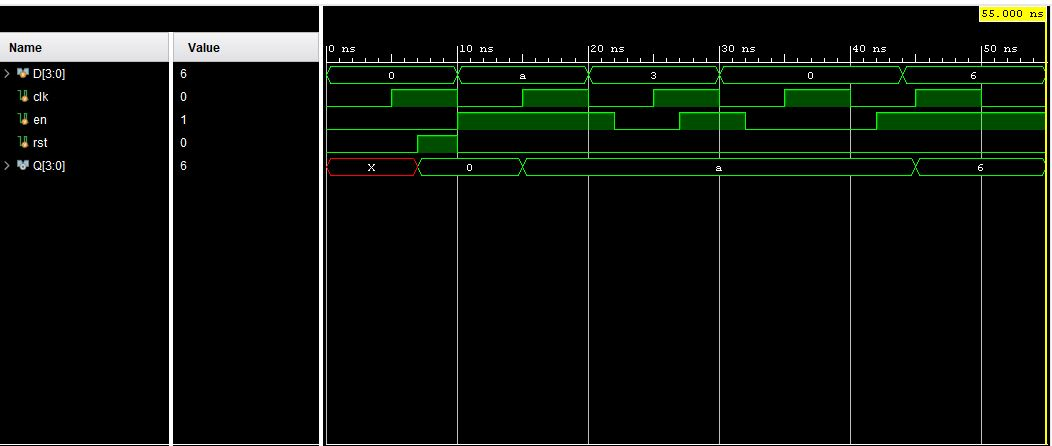
\includegraphics[width=1.0\textwidth]{Register Module}
	\caption{register expected results table and simulation}
	\label{fig:sim_with_table}=
\end{figure}
\clearpage


\begin{figure}[ht]\centering
	\begin{tabular}{l|rrrrrr}
		Time (ns): & 0-10 & 10-20 & 20-30 & 30-40 & 40-50 & 50-60 \\
		\midrule
		in0 & 01 & 00 & 01 &00  & 00 & 01 \\
		in1 & 01 & 00 & 00 & 01 & 00 & 01 \\
		op    & 0 & 1 & 2 & 3 & 4 & 5 \\
		\midrule
		out & 02 & 00 &00  & 01 & 00 & 01 \\
		\bottomrule
	\end{tabular}
	
	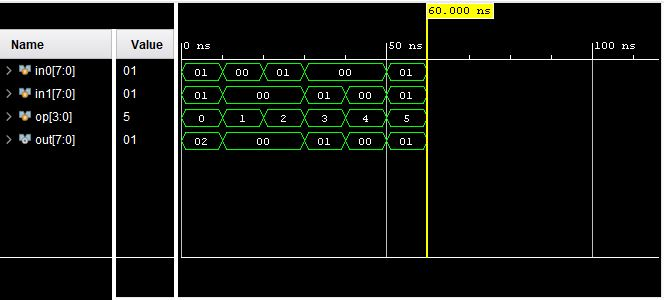
\includegraphics[width=1.0\textwidth]{ALU Module}
	\caption{ALU expected results table and simulation}
	\label{fig:sim_with_table}=
\end{figure}
\clearpage


\begin{figure}[ht]\centering	
	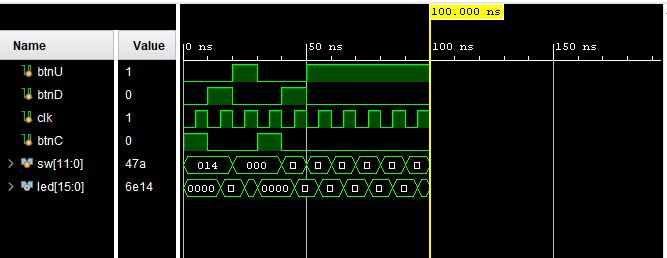
\includegraphics[width=1.0\textwidth]{Top Module}
	\caption{Top Level Simulation}
	\label{fig:sim_with_table}=
\end{figure}


\section*{Code}

\begin{lstlisting}[style=Verilog,caption=Register Source File ,label=code:ex ]

// Chris Jones , ELC 2137, 2020 -3-30-20

module register #(parameter N=1) 
(
input clk, rst, en, 
input [N-1:0] D, 
output reg [N-1:0] Q
);

always @( posedge clk , posedge rst )
begin
if (rst ==1)
Q <= en ; 
else if (en==1) 
Q <= D ;
end
// Notes:  
// - Reset is asynchronous , so this 
// block needs to execute when rst 
// goes high. 
// - We want enable to be synchronous 
// (i.e. only happens on rising 
// edge of clk), so it is left out 
// of "sensitivity" list.
endmodule


\end{lstlisting}

\begin{lstlisting}[style=Verilog,caption=Register Test Bench Code ,label=code:ex ]

// Chris Jones , ELC 2137, 2020 -3-30-20

module register_test();

reg [3:0] D;
reg clk, en, rst; 
wire [3:0] Q;

register #(.N(4)) r(.D(D), .clk(clk),
.en(en), .rst(rst), .Q(Q) );


// clock runs continuously 
always begin
clk = ~clk; #5; 
end

// this block only runs once
initial begin
clk=0; en=0; rst=0; D=4'h0; #7;
rst = 1; #3 //reset
D = 4'hA; en = 1; rst = 0; #10; 
D = 4'h3; #2; 
en = 0; #5; 
en = 1; #3; 
D = 4'h0; #2; 
en = 0; #10; 
en = 1; #2; 
D = 4'h6; #11; 
$finish;
end
endmodule




\end{lstlisting}



\begin{lstlisting}[style=Verilog,caption= Alu Source File,label=code:ex ]

// Chris Jones , ELC 2137, 2020 -3-30-20

module alu #(parameter N=8) 
(
output reg[N-1:0] out, 
input [N-1:0] in0, 
input [N-1:0] in1, 
input [3:0] op 
);

//Local parameters
parameter ADD=0; 
parameter SUB=1; 
parameter AND=2; 
parameter OR=3; 
parameter XOR=4;

always @* 
begin
case(op)
ADD: out = in0 + in1; 
SUB: out = in0-in1;
AND: out = in0 * in1;
OR: out = in0|in1;
XOR: out = in0^in1;// add the remaining commands 
default: out = in0;
endcase
end

endmodule

\end{lstlisting}


\begin{lstlisting}[style=Verilog,caption= Alu Test Bench ,label=code:ex ]
// Chris Jones , ELC 2137, 2020 -3-30-20

module ALU_test();
reg[7:0] in0;
reg[7:0] in1;
reg[3:0] op;
wire [7:0] out;
alu #(.N(8))a(.in0(in0),.in1(in1),
.op(op),.out(out));

initial begin
op = 0; in0 = 1; in1 = 1; #10;
op = 1; in0 = 0; in1 = 0; #10;
op = 2; in0 = 1; in1 = 0; #10;
op = 3; in0 = 0; in1 = 1; #10;
op = 4; in0 = 0; in1 = 0; #10;
op = 5; in0 = 1; in1 = 1; #10;
$finish;
end
endmodule

\end{lstlisting}



\begin{lstlisting}[style=Verilog,caption=Top Level Source File,label=code:ex ]
//Chris Jones , ELC 2137, 2020 -3-30-20

module top_lab9(
input clk, btnC, btnD, btnU,
input [11:0] sw,
output reg[15:0] led
);
wire [7:0] A1;
wire [7:0] R1;


register #(. N (8) ) r1 (. D(sw[7:0]),. clk(clk) ,. en(btnD),.rst(btnC),.Q(R1));

alu #(.N(8)) a(.in1(R1),.in0(sw[7:0]),.op(sw[11:8]),.out(A1));

register #(.N(8))r2(.D(A1),. clk(clk) ,. en(btnU) ,. rst(btnC),. Q(led[15:8]));

assign led[7:0] = R1;
endmodule

\end{lstlisting}






\end{document}

